\section{Software Microcontrollore}
Il codice per la programmazione del microcontrollore si sviluppa dall'applicazione di base "\textit{LoRaWAN\_End\_Node}" che fornisce
le funzioni necessarie per l'inizializzazione dei componenti nececessari e la comunicazione del microcontrollore attraverso il protocollo LoRa.
\\\\Per poter leggere i dati che si intendono acquisire dai sensori si è reso necessario organizzare e riformulare parte di codice per l'inizializzazione e il funzionamento dell'accelerometro
e del giroscopio. Nelle sezioni \ref{ssec:sensori} e \ref{ssec:lorawan} vengono rispettivamente presentate la strategia di collegamento e lettura dei sensori selezionati e 
le modifiche apportate al codice per poter comunicare correttamente con il cloud.

\subsection{Lettura sensori}\label{ssec:sensori}
% BREVE SCALETTA:
% 1) Descrizione breve del collegamento hardware e del bus I2C

% 2) Descrizione delle funzioni per l'inizializzazione e l' acquisizione dei sensori dall'almbiente esterno
% -Cenno a LSM6DSO_USER_Init() e la sua posizione nel codice
% -Cenno LSM6DSO_USER_Acc_GetAxes() e LSM6DSO_USER_Gyro_GetAxes()
Per leggere i dati misurati dall'accelerometro e dal giroscopio, sono state sviluppate due funzioni in particolare (riportate in Figura \ref{fig:lettura_sensori}). Queste due funzioni leggono i dati dell'accelerometro e del giroscopio rispettivamente e restituiscono un "exit code" uguale a zero se la lettura è stata completata con successo e i valori letti vengono scritti sulle tre variabili passate tramite puntatore.
\begin{figure}[h!]
  \centering
  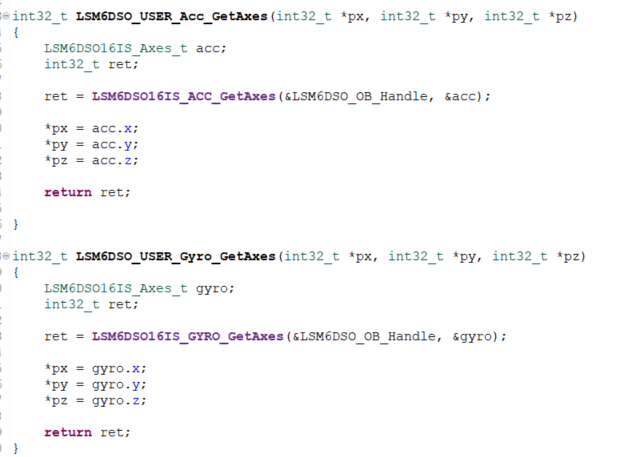
\includegraphics[width=0.9\textwidth]{getDataFunctions.png}
  \caption{Funzioni di lettura dei sensori}
  \label{fig:lettura_sensori}
\end{figure}
\\Affinché queste funzioni operino correttamente, è necessario chiamare le seguenti funzioni:
\begin{itemize}
  \item \Verb|LSM6DSO_USER_Init()| all'interno della funzione \Verb|LoRaWAN_Init| (dichiarata nel file \textit{lora\_app.c})
  \item \Verb|BSP_I2C2_Init()| nel \textit{main.c}
\end{itemize}
% 3) Descrizione della funzione EnvSensorRead() e della struttura dati sensor_data per la lettura del sensore
I dati che si intendono inviare al cloud sono racchiusi nella variabile \Verb|sensor_data| (presente in Figura \ref{fig:envsensorread}) di tipo \Verb|sensor_t|. La struttura di \Verb|sensor_t| è riportata in Figura \ref{fig:sensor_t} ed è stata modificata aggiungendole i campi \Verb|acc_x|, \Verb|acc_y| e \Verb|gyr_y|, necessari al funzionamento del nostro sistema.
\begin{figure}[h!]
  \centering
  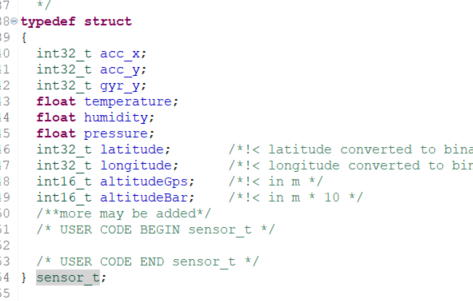
\includegraphics[width=0.7\textwidth]{sensor_t.png}
  \caption{Struttura dati sensor\_t}
  \label{fig:sensor_t}
\end{figure}
\\La funzione \Verb|EnvSensorRead| (riportata in Figura \ref{fig:envsensorread}) legge i dati dei sensori e li scrive nella variabile \Verb|sensor_data| (passata tramite puntatore). Questi dati saranno poi processati nella funzione \Verb|SendTxData| (vedi Sezione \ref{sssec:uplink_scheda}).
\begin{figure}[h]
  \centering
  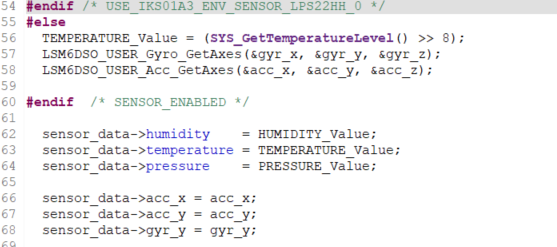
\includegraphics[width=0.9\textwidth]{EnvSensorRead.png}
  \caption{Parte della funzione EnvSensorRead}
  \label{fig:envsensorread}
\end{figure}

\subsection{LoRaWAN}\label{ssec:lorawan}
% Breve descrizione del protocollo di rete
% -LoRaWAN_Init() per l'aggiornamento delle variabili
% -Cenno al DutyCicle per il tempo di lettura delle variabili? --> 3-4s ottimale
% File utili: main.c app_lorawan.c lora_app.c sys_sensor.h sys_sensor.c

  \subsubsection{Uplink scheda}\label{sssec:uplink_scheda}
  % Descrizione della funzione SendTxData
  % -Riferimento a variabile roll_state per decidere che dati inviare
  % -Strategia operativa per inserire i dati di sensor_data nel buffer


  \subsubsection{Downlink scheda}
  % Descrizione della funzione OnRxData:
  % -Riferimento a Variabile roll_state
  % -Lettura del buffer
  % -Accensione del led sulla scheda e cambiamento di stato



